% Capitulo 2

\chapter{Estado del Arte} % Main chapter title

\label{EstadoDelArte} % For referencing the chapter elsewhere, use \ref{Chapter1} 

\lhead{Capítulo 2 \emph{Estado del Arte}} % This is for the header on each page - perhaps a shortened title

%----------------------------------------------------------------------------------------

Existen dos clases de aplicaciones que se analizaron: aplicaciones con localización en interiores y otras que brindan información sobre aeropuertos. Las Tablas \ref{tab:appsInteriores} y \ref{tab:appsViajes} muestran estas aplicaciones.

\definecolor{blanco}{RGB}{255,255,255}

\begin{table}[h]
	\begin{center}
		\begin{tabular}{|>{\color{blanco}}c|>{\color{blanco}}c|>{\color{blanco}}c|>{\color{blanco}}c|>{\color{blanco}}c|}
			\hline \rowcolor[RGB]{51,153,255} 
				{\bf Aplicación} & 
				{\bf Descripción} &
				{\bf Precio} &
				{\bf Plataforma(s)} &
				{\bf Logotipo} \\
			\hline 
				\multicolumn{1}{|m{1.8cm}|}{\centering Crux} &
				\multicolumn{1}{m{4.5cm}|}{Aplicación móvil que permite conocer la ubicación en interiores. Ofrece herramientas para potenciar las ventas, las visitas, la fidelidad de los clientes, la experiencia de compra y su grado de satisfacción. \cite{crux}} &
				\multicolumn{1}{m{1.05cm}|}{\centering Gratis} &
				\multicolumn{1}{m{2.5cm}|}{\centering Android} &
				\multicolumn{1}{m{2.5cm}|}{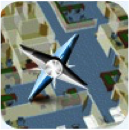
\includegraphics[width=25mm, height=25mm]{Figuras/crux.png}} \\
      		\hline \rowcolor[RGB]{240,248,255} 
      			\multicolumn{1}{|m{1.8cm}|}{\centering Meridian} &
				\multicolumn{1}{m{4.5cm}|}{Guía a los viajeros paso a paso hacia el lugar que deseen visitar dentro del aeropuerto. Integra bases de datos de las tiendas en el aeropuerto, horarios de vuelos y cuentas de redes sociales. \cite{meridian}} &
				\multicolumn{1}{m{1.05cm}|}{\centering Gratis} &
				\multicolumn{1}{m{2.5cm}|}{\centering iOS y Android} &
				\multicolumn{1}{m{2.5cm}|}{
\includegraphics[width=25mm, height=25mm]{Figuras/meridian.png}} \\
      		\hline 
		\end{tabular}
	\end{center}
	\caption[Aplicaciones para Localización en Interiores]{Aplicaciones para Localización en Interiores} 
	\label{tab:appsInteriores}
\end{table}

\begin{table}[h]
	\begin{center}
		\begin{tabular}{|>{\color{blanco}}c|>{\color{blanco}}c|>{\color{blanco}}c|>{\color{blanco}}c|>{\color{blanco}}c|}
			\hline \rowcolor[RGB]{51,153,255} 
				{\bf Aplicación} & 
				{\bf Descripción} &
				{\bf Precio} &
				{\bf Plataforma(s)} &
				{\bf Logotipo} \\
			\hline 
				\multicolumn{1}{|m{1.8cm}|}{\centering GateGuru} &
				\multicolumn{1}{m{4.5cm}|}{Recibe datos de unos 180 aeropuertos ubicados en EE.UU., Canadá, Europa y Asia, de tal forma que da a conocer el estado de vuelos. La aplicación también permite visualizar itinerarios conectándose con Tripit y Kayak. Además de obtener mapas, información sobre el clima y alquileres de coche. \cite{gateguru}} &
				\multicolumn{1}{m{1.05cm}|}{\centering Gratis} &
				\multicolumn{1}{m{2.5cm}|}{\centering iOS, Android y Windows Phone} &
				\multicolumn{1}{m{2.5cm}|}{
\includegraphics[width=25mm, height=25mm]{Figuras/gateGuru.png}} \\
      		\hline \rowcolor[RGB]{240,248,255} 
      			\multicolumn{1}{|m{1.8cm}|}{\centering Kayak} &
				\multicolumn{1}{m{4.5cm}|}{Es un gran buscador que ahora ha pasado a ser también una aplicación. Con Kayak se pueden comparar ofertas de vuelo, hoteles y alquileres de coches, así como buscar tarifas de equipajes; acceder a los teléfonos de las aerolíneas y a la información de los aeropuertos. \cite{kayak}} &
				\multicolumn{1}{m{1.05cm}|}{\centering Gratis} &
				\multicolumn{1}{m{2.5cm}|}{\centering iOS, Android, Windows Phone y Kindle Fire.} &
				\multicolumn{1}{m{2.5cm}|}{
\includegraphics[width=25mm, height=25mm]{Figuras/kayak.png}} \\
      		\hline
      			\multicolumn{1}{|m{1.8cm}|}{\centering Tripit} &
				\multicolumn{1}{m{4.5cm}|}{Es un organizador de viajes que se puede usar desde el teléfono o la tableta en conexión directa con tripit.com. Además la aplicación alerta sobre posibles retrasos de vuelos y cuenta con un  despertador, muy útil si se viaja temprano. \cite{tripit}} &
				\multicolumn{1}{m{1.05cm}|}{\centering \$ 49 anual} &
				\multicolumn{1}{m{2.5cm}|}{\centering iOS, Android, Blackberry y Windows Phone.} &
				\multicolumn{1}{m{2.5cm}|}{
\includegraphics[width=25mm, height=25mm]{Figuras/tripit.png}} \\
      		\hline
			\end{tabular}
	\end{center}
	\caption[Aplicaciones con Información de Viajes]{Aplicaciones con Información de Viajes} 
	\label{tab:appsViajes}
\end{table}

\newpage
En la Tabla \ref{tab:publicacionesInteriores} se muestra una recopilación de las publicaciones que se han desarrollado sobre la localización en interiores.

\begin{table}[h]
	\begin{center}
		\begin{tabular}{|>{\color{blanco}}c|>{\color{blanco}}c|>{\color{blanco}}c|}
			\hline \rowcolor[RGB]{51,153,255} 
				{\bf Artículo} & 
				{\bf Autores} &
				{\bf Resumen} \\
			\hline 
				\multicolumn{1}{|m{4cm}|}{\centering ILS (Indoor Location Systems) Sistemas de Localización en Interiores} &
				\multicolumn{1}{m{4.5cm}|}{\centering Raúl Sánchez Vítores} &
				\multicolumn{1}{m{4.5cm}|}{Este trabajo presenta los problemas existentes de la localización en interiores para después presentar una clasificación de los sistemas ILS y las distintas soluciones técnicas que se han desarrollado. \cite{ILS}} \\
      		\hline \rowcolor[RGB]{240,248,255} 
      			\multicolumn{1}{|m{4cm}|}{\centering Uso del campo magnético de la tierra para localizar a las personas en interiores} &
				\multicolumn{1}{m{4.5cm}|}{\centering Carlos Eric Galván Tejada \newline
				Juan Pablo García Vázquez \newline
				Jorge Isaac Galván Tejada} &
				\multicolumn{1}{m{4.5cm}|}{Este trabajo explica las técnicas que se emplean para localizar en interiores utilizando el campo magnético y menciona las ventajas que se tienen a comparación de otras formas de realizar la localización en interiores. \cite{usoCampoMagnetico}} \\
      		\hline 
		\end{tabular}
	\end{center}
	\caption[Publicaciones sobre Localización en Interiores]{Publicaciones sobre Localización en Interiores} 
	\label{tab:publicacionesInteriores}
\end{table}